%---------------------------------------------------------------------------------
\chapter{A Novel Architecture for Multiple Standard Cognitive Radios}
\label{chap:MSCR}
%---------------------------------------------------------------------------------

%---------------------------------------------------------------------------------
\section{Introduction and Related Works}
%---------------------------------------------------------------------------------
Cognitive radios that support multiple bands, multiple standards and adapt operation according to environmental conditions are becoming more attractive as the demand for higher bandwidth
and more efficient spectrum use increases. 
Traditional implementations in custom ASICs cannot support such flexibility, with standards changing at a faster pace, while software implementations of baseband communications fail to achieve the performance required.
Hence, FPGAs offer an ideal platform bringing together flexibility, performance, and efficiency.

Most practical CRs are built using powerful general purpose processors to achieve flexibility through software, but they can fail to offer the computational throughput required for advanced modulation and coding techniques and they often have high power consumption.
GNU Radio~\cite{gnuradio} has been a widely used platform in academia. 
It is a software application that runs on a computer or an embedded ARM processor platform, e.g. on the Ettus USRP E100. 
Computational limitations mean that while it has been successful for investigating CR ideas, it is not feasible for implementing advanced embedded radios using complex algorithms.
Other software based frameworks like Iris~\cite{Sutton2010}, have some limited support for FPGAs but suffer from poor bandwidth between software and hardware.
Moreover, the compilation time and reconfiguration time of software defined radio based system are quite long for CRs may not be suitable for adapting fast condition changing requirements.

In an application area with fast moving standards and requiring support for multiple standards, custom ASIC implementation is both unlikely to be agile or cost effective enough to cope with fast-changing standards and operating requirements. 
In order to address this, Delorme et al.~\cite{Delorme2008} presented a heterogeneous reconfigurable hardware platform for Cognitive Radio. 
It can adapt its hardware structure to support standards like GSM, UMTS, and wireless LAN. 
Most processing components run as embedded software on the nodes in a network on chip processor, while the channel coder and the mapping of the RX chain are implemented inside an FPGA. 
Partial reconfiguration (PR) is used to switch the channel coder from one context to an another depending on SNR. 
A processor manages data movement between the different processors, the ASIC, and the FPGA. The need for a large data buffer and inefficient data transfer mechanisms lead to increased power consumption and reduced throughput.
There are few studies on FPGA based platforms for radio implementation. 
KUAR~\cite{Minden2007} is a mature radio platform built around a fully-featured Pentium PC with a Xilinx Virtex II FPGA. 
The baseband processing is accelerated on FPGA and only limited for NC-OFDM signal based on the IEEE 802.16 standard.
Projects at Virginia Tech~\cite{athanaswires} have shown dynamically assembled radio structures on FPGAs, where the target radio system is defined at a high-level with datapaths connecting relatively large functional modules. 
The modules are wrapped, and each of them consists of a PR module with complied partial bit-streams stored in dynamic library. 
Using PR eliminates the need for run time compilation, thus affording flexibility. 
A flexible radio controller can insert and remove compiled modules to adapt to current conditions.

Our proposed research focuses on designing the baseband processing of a MSCR system.
This work explores the advantages of coupling PR and parameterised functional units in one architecture to offer flexibility for OFDM-based baseband processing while minimising reconfiguration time. 
To the best of our knowledge, there is no published research on dynamical reconfiguration for OFDM-based baseband processing of multiple standards cognitive radio on FPGA.

%---------------------------------------------------------------------------------
\section{Proposed OFDM-based baseband modulation for MSCR}
%---------------------------------------------------------------------------------
\begin{figure}
\centering
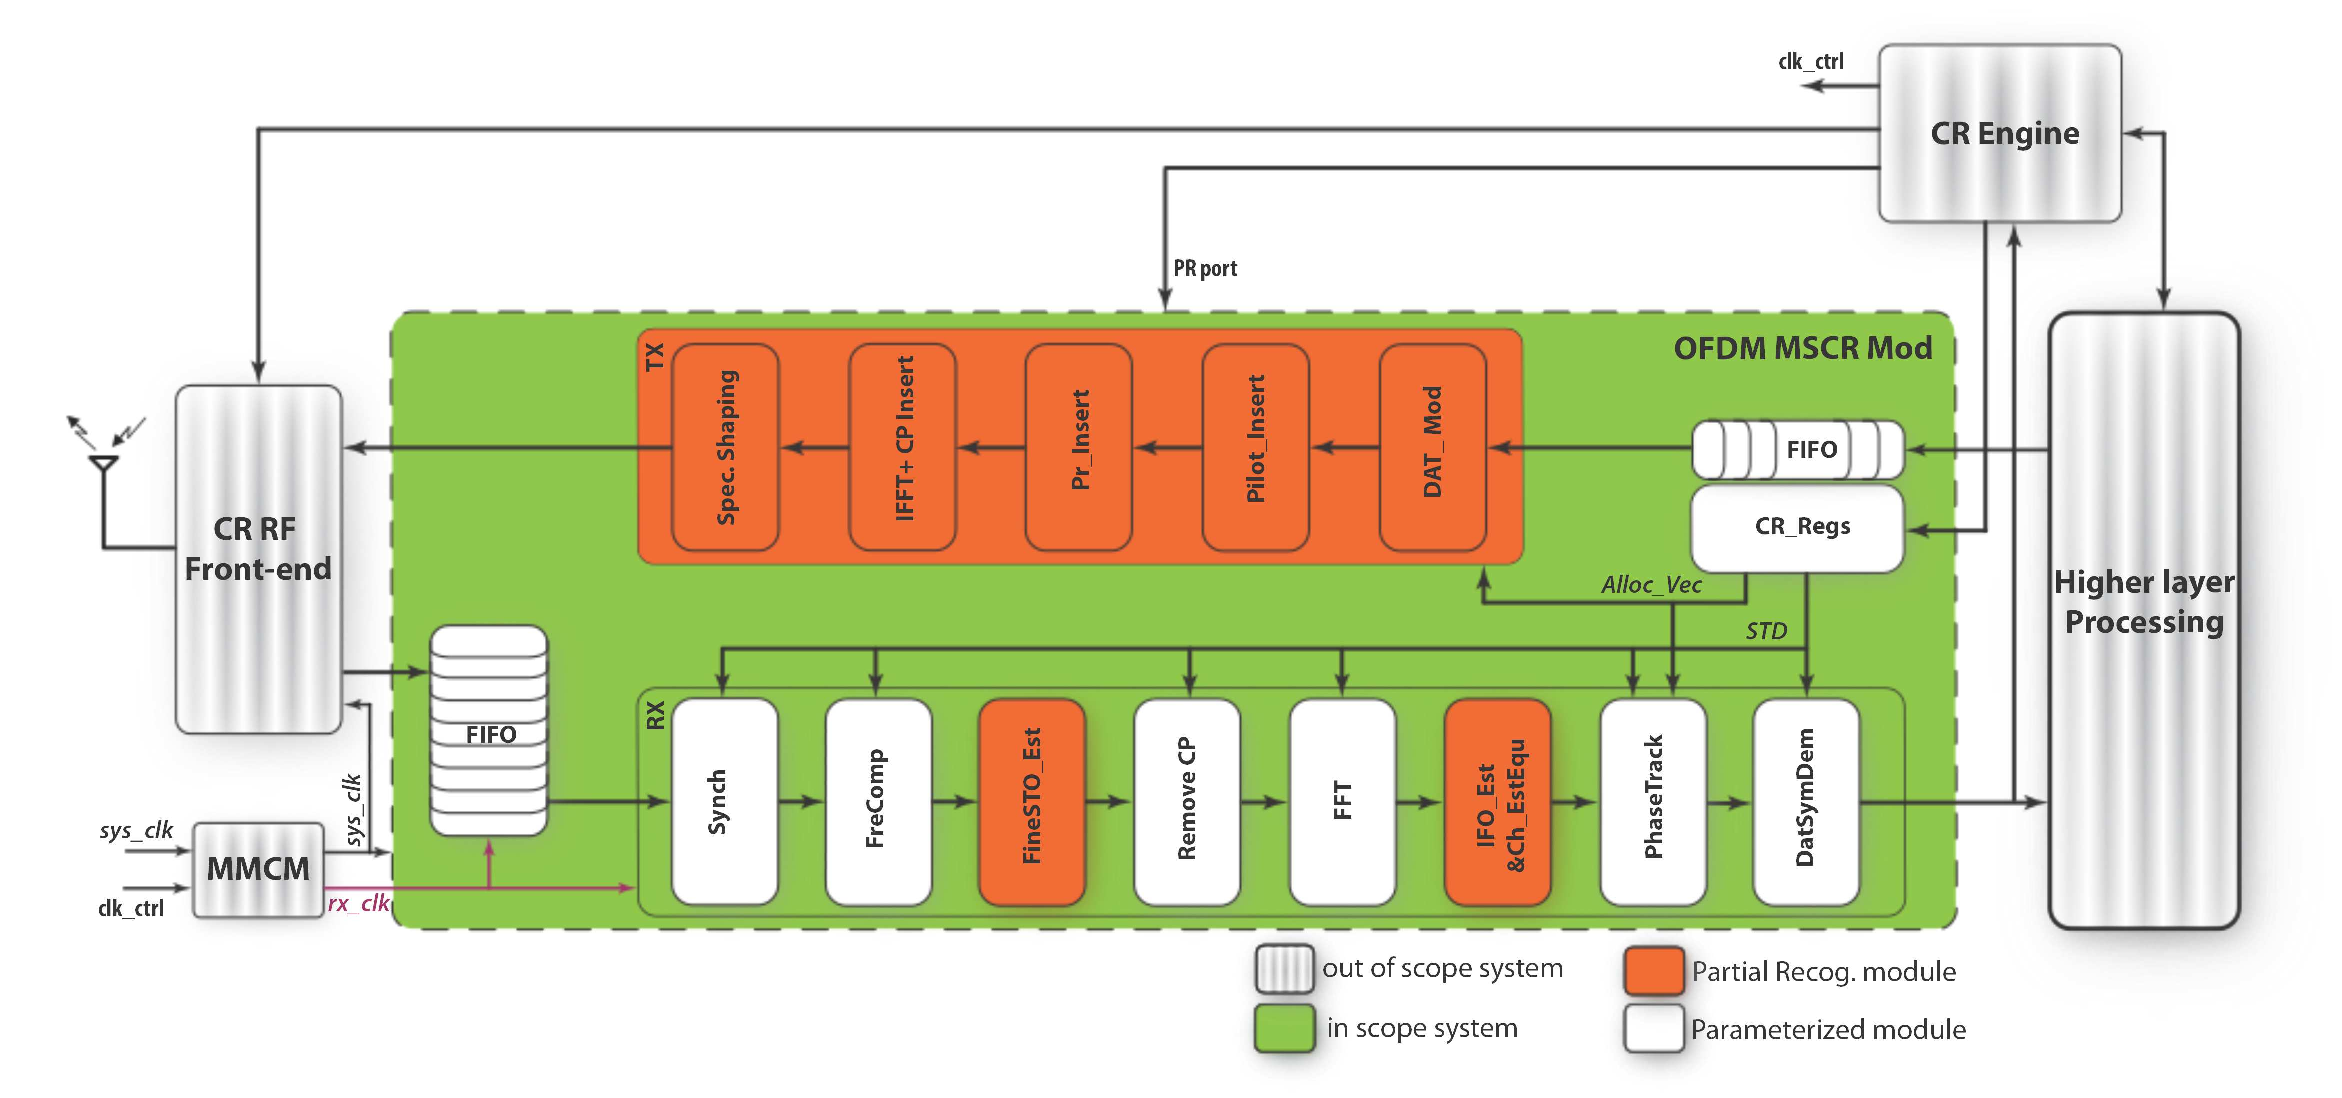
\includegraphics[width=1\columnwidth]{Figures/MSCRFig.pdf}
\caption{The structure of a generic MSCR system}
\label{fig:struc}
\end{figure}

Fig.~\ref{fig:struc} illustrates the proposed structure of baseband modulation for our OFDM-based MSCR. 
A mix of partially reconfigurable and parameterised modules make up the baseband implementation.
FIFOs are included to help overcome the reconfiguration latency when PR modules are reconfigured. 
Since these modules are now just a small part of the system, buffering is significantly reduced over a more general implementation.

	\subsection{System Description}

We developed a prototype MSCR baseband modulation that supports transceiving non-contiguous OFDM (NC-OFDM) signals.
This system can perform with different OFDM symbol lengths and frame formats specified differently according to multiple standards such as IEEE~802.11~\cite{IEEE80211}, IEEE~802.16~\cite{IEEE80216}, and IEEE~802.22~\cite{IEEE80222}.
The main specifications of these standards are summarised in Table~\ref{Tab:spec}.

\begin{table}[h]
\label{Tab:spec}
\centering
\caption{System specifications of three supported OFDM-based standards.}{
\renewcommand{\arraystretch}{1.3}
\begin{tabular}{@{}llll@{}}
\toprule
Specifications 			& IEEE~802.11 				& IEEE~802.16				& IEEE~802.22 		\\ \midrule
Frequency band			& 2.4--2.5~GHz				& 5--6~GHz					& 54--862~MHz		\\
Channel Width			& 10~MHz					& 10~MHz					& 8~MHz			\\
Sampling Frequency		& 10~MHz					& 11.52~MHz				& 9.136~Mhz		\\
FFT size ($N_{FFT}$)		& 64						& 256						& 2048			\\
CP Length				& 16						& 32						& 512				\\
Number of data carriers		& 48						& 192						& 1440			\\
Number of pilots			& 4						& 8						& 240				\\ 
\end{tabular}
}
\end{table}

Basically, The CR implementation is divided into a control plane and data plane. 
The data plane performs data processing for the radio system in data stream. 
It tranceives data streams to/from the RF front end through two AXI (Advanced eXtensible Interface) stream interfaces.
For transmission, sending data from higher level layers is processed and modulated by the data plane.
Then modulated sample streams are transferred to RF front end to convert to analogue signals and subsequently be up-converted to RF band before transmission on the RF channel.
For the receiver side, the received signals are down-converted to the baseband followed by analogue to digital convertion form a sample stream.
The sample stream is demodulated and processed at the data plane before transferring to a higher level layer.
To support multiple standards, the data plane has to provide the flexibility of switching functions accordingly to the parameters specified in different standards.
The AXI stream interfaces are used for the overall data plane system as well as each sub-module.
This unified interface is required to make partial reconfiguration possible, since modules that are reconfigured should share the same connections.
This interface also allows the data from higher layers to be processed in a streaming format. 
This reduces the requirement for buffering, hence optimising resource usage and total power consumption~\cite{Liu2009}. 
Each module has one slave interface to receive data from the previous module and one master interface to send processed data to the subsequent module.

The control plane is a cognitive radio (CR) engine that is required to perform the adaptive algorithm based on sensing data from the receiver to decide the allocation vector and the required standard.
It monitors events in the data plane via an AXI bus interface connected set of registers. 
The control plane needs to issue commands to the data plane through the same bus register interface. 
In addition, the CR engine consists of the PR controller that is responsible for download the pre-complied bitstreams stored in DRAM into the corresponding PR modules through the ICAP (Internal Configuration Access Port) interface~\cite{Vipin2012} when the CR engine decides to change the standard.
The control plane can be implemented in one of a number of ways. 
It can be standalone software running on a processor core. It can also be hardware in a separate part of the FPGA. 
Alternatively, for maximum flexibility and programming support, it can run on top of an operating system on the processor.
By ensuring that symbol data is processed and moved through the data plane independently of the processor in the control plane, we are able to achieve a high throughput. 
Normally, the data plane processes data streams based on a specified standard to transceive data symbols according to the allocation vectors.
The CR engine must be able to performs sensing and adaptive tasks to update suitable allocation vectors based on current channel status.
When the frequency band of the current operating standard is mostly occupied by PUs and IUs, the CR engine performs switching to an other standard or frequency band that is currently (or will soon be) free for transmission.
The PR controller inside the CR engine is required to download the bitstreams of PR modules according to the new standard.
In the meantime, the CR engine configures the system by writing relevant parameters to registiters in $CR\_Regs$ such as allocation vectors (Alloc\_vec), symbol modulation type (MOD), and standard (STD).

The scope of this chapter focuses on the baseband modulation in order to deal with the challenges of long configuration. 
The system takes the advantages of coupling PR and parameterised functional units to offer flexibility while minimising reconfiguration time.
The CR system is assumed capable of performing in burst mode in which the system only transmit the packages as soon as data is available~\cite{Ai2006}.
The transmitter subsystem just performs the transmission initiated by the higher layer.
If the system needs to transmit data during the periods of reconfiguration time, the data package will be stored in FIFO. 
The stored data packet will be flushed out of FIFO for transmission after the reconfiguration of the transmitter has been done.
Moreover, the hardware usage for the transmitter side is so small compared to the receiver side that it has a much faster reconfiguration time.
The hardware usage and reconfiguration time of the transmitter is presented latter in Section~\ref{sec:PerAna}.
The reconfiguration time does not cause a critical disruption of the processing chain and loss of transmitted packets.
Therefore, the monolithic PR module for the transmitter side is implemented because of simplicity and flexibility.
In contrast, the receiver subsystem is required to continuously the receive signal and detect the data frame.
Furthermore, the hardware usage for the receiver subsystem is very large resulting in a long reconfiguration time.
To avoid losing data frames, a huge FIFO is required to store received samples from the RF front end during reconfiguration and this is not practical.
The critical  issue is to minimise the reconfiguration time in the receiver subsystem in an attempt to achieve these aims.
The coupling of PR and parameterised functional units is applied to implement the receiver subsystem. 
The design of each module in the receiver subsystem to obtain the flexibility, while minimising reconfiguration time, will be investigated in the next subsection.
In addition, after reconfiguring the receiver subsystem, the FIFO needs to be flushed for the next reconfiguration. 
A Mixed-Mode Clock Manager (MMCM) is employed to increase the received processing rate (rx\_clk).
After stored samples for reconfiguration are read out, the received processing rate is reduced to the sampling rate (sys\_clk) to reduce power consumption.
The MMCM module is also required to change the processing rate of data plane according to the different samppling rates specified in different standards, shown in Table~\ref{Tab:spec}.

	\subsection{Module Description}

In this subsection, each functional module, shown in Fig.~\ref{fig:struc}, in the receiver processing chain is investigated and commonalities across standards are analysed.
In term of design options, there is a tradeoff between the simplicity, flexibility, and long reconfiguration latency of PR module and the increased hardware overhead, complexity, but faster configuration of parameterised modules.
The comparison between the hardware usage of parameterised modules for multiple standards and that of individual specified standard modules is evaluated.
If the hardware overhead required to parameterise the module is less than given percentage above the hardware size of the standard-alone module, then it is judged better to be parameterised.  
For those modules that require significant changes (i.e. the parameterised overhead is greater than this threshold) or are required to support unspecified parameter for future standard (such as preamble), PR can be used on a per-module level. 
The bistream for each standard is implemented and precompiled separately.
As a result, when switching from one standard to another, only part of the FPGA needs to be reconfigured.

\begin{enumerate}

\item {FIFO buffer (FIFO):}
There are two FIFOs at the transmitter side and the receiver side to buffer the data sent from the higher layer and the RF front end, respectively.
The FIFO buffers are implemented based on the FIFO IP cores with 2 port AXI stream interface configuration.
In the normal operation of data stream, one data word is written to the buffer by the higher layer/the RF front end, meantime, another one is read out from the buffer by the transmitter side/ the receiver side at every single system clock.
Therefore, the FIFO buffers normally operate in almost empty state.
When the reconfiguration is required for switching underlying standard, the transmitted processing and received processing are suspended processing data streams. 
The FIFO buffers are stored coming data streams to avoid losing frames.
Because the system performs in burst mode, the trasmitted streams are not continuously, therefore, the transmitted FIFO can be flushed the stored data during the gap of the burst streams.
The data buffer is not a critical issue for the transmitter side.
However, the receiver side needs to continuous processing data streams from the RF front end to detect incoming frames. 
The receiver side does not have spare time to flush the stored data in FIFO bufferred during reconfiguration time.
Therefore, the received FIFO is configured with independent clocks as shown in the Fig.~\ref{fig:FIFO}. 
In order to flushing stored data in the received FIFO after switching standard reconfiguration, the MMCM increases the received processing rate (rx\_clk) be multiple time greater than the sampling rate of the RF front end to make the FIFO be almost empty for the next reconfiguration.
When the received FIFO is almost empty the received processing rate is reduced back to equals the sampling rate to minimise power consumption.
\begin{figure}
\centering
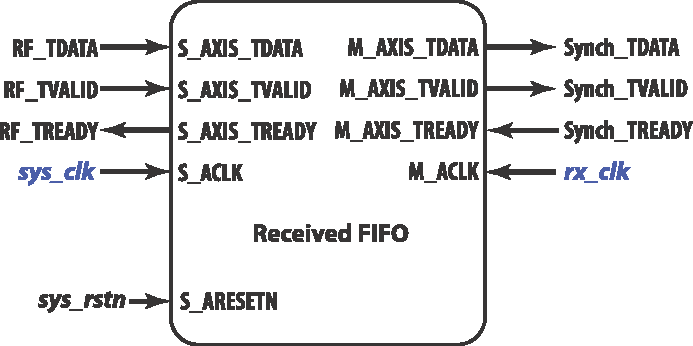
\includegraphics [width=0.5\columnwidth]{Figures/MSCR_RX_FIFO.pdf}
\caption{The received FIFO module}
\label{fig:FIFO}
\end{figure}

\item {Synchronisation (Synch):}
The CR system performs in burst mode.
\emph{Synch} is to detect the presence of a frame and estimate the frequency offset required, based upon the preamble of the received frame.
This module performs estimation based on the timing parameters, defined by Schmidl and Cox \cite{Schmidl1997}, expressed as below;
\begin{center}
\begin{eqnarray}
\label{MMetric}
P[d] &=&\sum_{m =0}^{L-1}    (r^{*}[d+m]r[d+m+L] ) \nonumber \\
R[d] &=&\sum_{m =0}^{L-1}   |r[d+m+L]|^2 \nonumber \\
M[d] &=& \frac{|P[d]|^2} {(R[d])^2},
\end{eqnarray}
\end{center}
where $d$ denotes a time sequential index of received samples $r$, $L$ is the periodic length of the short preamble, $^*$ denotes complex conjugation.

As discussed in Chapter~\ref{chap:Synchronisation}, the frame detection is performed by finding the plateau of $M$ when a frame presents at receiver.
$P$ is also used to estimate fractional CFO in the subsequent module. 
The Fig.~\ref{fig:Sync} shows block diagram of synchronisation implementation.  
The timing metrics are calculated by using auto-correlation on received samples.
\emph{Coarse Time} detects the new frame and estimate roughly the start of frame based on the comparison the metric $P$ and the value $\frac{R}{2}$ that is equivalents to detect M greater than a threshold of 0.25.
The method is blind estimation that provides a generality to be applied for multiple standards.
By parameterising the length of $L$, the synchronisation module can effectively perform for three current supported standards as well as be extensible for future standards.
Therefore, this module is implemented as a parameterised version with parameter $L$ whose values are defined together with the length of FFT ($NFFT$), shown in Table~\ref{Tab:L}.
The parameterised value combinations of $L$, and $NFFT$ allow for the support of multiple standards.
The parameterised values consist not only of the required combinations for 802.11, 802.16, and 802.22, but also support other combinations for future standards.
\begin{table}[h]
\centering
\caption{Parameterised values according to supported standards}{
\begin{tabular}{|l||*{6}{c|}}\hline
\theadset\theadfont\backslashbox[3em]{NFFT}{L}
&\makebox[2.3em]{\thead{16}}&\makebox[2.3em]{\thead{32}}&\makebox[2.3em]{\thead{64}} &\makebox[2.3em]{128}&\makebox[2.3em]{\thead{256}}&\makebox[2.3em]{\thead{512}}\\\hline\hline
64 		& 802.11 & & & & & \\\hline
128 	& & & & & & \\\hline
256 	& & & 802.16 & & & \\\hline
512 	& & & & & & \\\hline
1024 	& & & & & & \\\hline
2048 	& & & & & & 802.22\\\hline
\end{tabular}
\label{Tab:L}
}
\end{table}

\begin{figure}
\centering
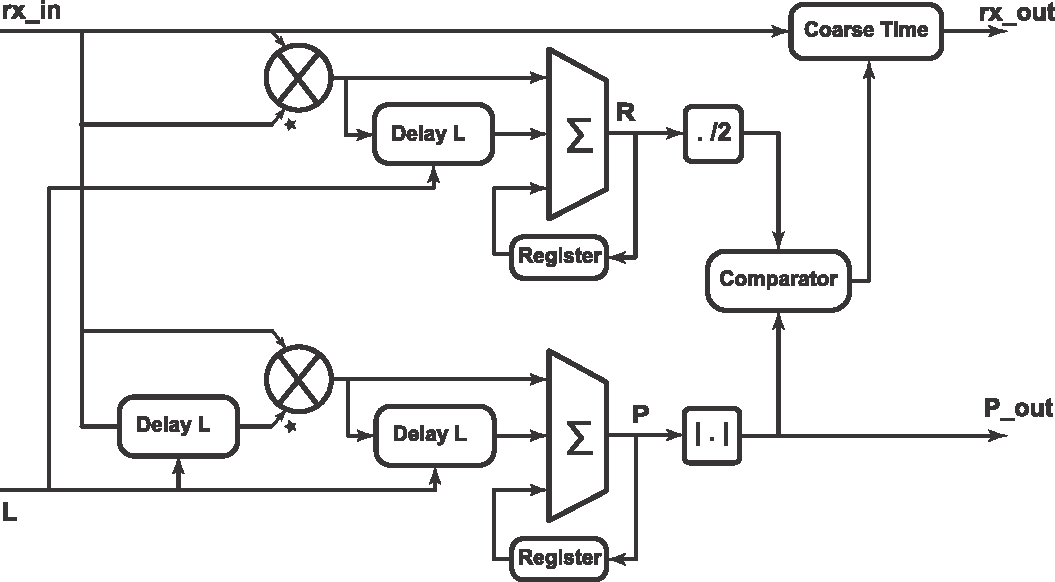
\includegraphics [width=0.9\columnwidth]{Figures/MSCR_RX_Sync.pdf}
\caption{The block diagram of Synchronisation module}
\label{fig:Sync}
\end{figure}

\item{Frequency Compensation:}
\emph{FreComp} module performs fractional CFO estimation based on the value of $P$ passed from the previous module \emph{Synch}. 
Fractional CFO estimation and compensation are mathematically expressed as below;
\begin{eqnarray}
\label{fractionalCFO}
\widehat{\Delta f } &=& \frac{\angle P}{2\pi L} \nonumber \\
\widehat{r[d]} &=& r[d] e^{-j2\pi\widehat{\Delta f} d}
\end{eqnarray}
where $\widehat{\Delta f }$ is estimated fractional CFO, $\angle P$ denotes the angle of P and $N$ is number of FFT points.

The Fig.~\ref{fig:FFO} illustrates the block diagram of frequency compensation. 
A phase rotation sub-module is used to compensate fractional CFO by rotating the received sample phase with a proper angle.
The proper angles are calculated and accumulated based on estimated fractional CFO.
\begin{eqnarray}
\label{AccumCFO}
\phi[d] &=& \phi[d-1] + \frac{\angle P}{L} \nonumber \\
\widehat{r[d]} &=& r[d] e^{-j \phi[d]}
\end{eqnarray}

According to (\ref{AccumCFO}), the computation of \emph{FreComp} depends on the periodic length of short preamble that is used to calculate $P$. 
Assuming that $L$ is normally defined with a power of two value, the division by $L$ can be effectively computed by a right shift.
Therefore, this module can be effectively implemented to support multiple standards by parameterising a right shifter according to the value of $L$. 
\begin{figure}
\centering
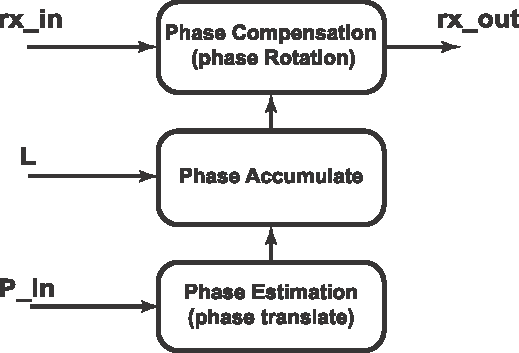
\includegraphics [width=0.5\columnwidth]{Figures/MSCR_RX_FFO.pdf}
\caption{The block diagram of frequency compensation module}
\label{fig:FFO}
\end{figure}

\item{Fine STO Estimation:}
\emph{FineSTO\_Est} is to estimate the starting sample of each OFDM symbol. 
The RF front-end for MSCR need to access a wide range of frequencies, shown in Table~\ref{Tab:spec}. Depending on the standard in operation, the CFO may be large, resulting in the present of IFO.
Therefore, the implementation of \emph{FineSTO\_Est} is based on the algorithm presented in \cite{Pham2014} that is also robust to IFO.
The metric of fine STO estimation is expressed as below;
\begin{equation}
\label{ProposedR}
S[d] =\sum_{m =0}^{L-1}   |r[d+m+L]|^2  |a[m]|^2,
\end{equation}
when $|a[m]|$ denotes the normalised amplitude of the preamble at the transmitter.
The Fig.~\ref{fig:STO} shows the block diagram of fine STO estimation.
The metric is calculated based on the multiplierless correlation between received samples and transmitted preamble.
The cross-correlation provides high precision for STO estimation. 
However, this operation requires a large number of DSP blocks, resulting in increased hardware resource and power consumption of the system.
Reducing the hardware resource and power consumption requires using multiplierless correlation \cite{Pham2012}.
\emph{Peak Detect} finds the maximum value of correlation that is employed to accurately estimate the STO and \emph{Fine Time} determines the exact first sample of the next OFDM symbol (long preamble symbol).
However, the multiplierless correlation is not flexible and depends on preambles that are different for each standard.
Therefore, we employ the PR module for the {FineSTO\_Est} module to obtain flexibility.
Each supported standard is implemented separately and precompiled to a stored bitstream.
The suitable precompiled bitstream will then be downloaded to the PR module by the \emph{CR engine} when the underlying standard is switched.
The PR module must evidently to be large enough to contain the largest bitstream among the supported standards.
\begin{figure}
\centering
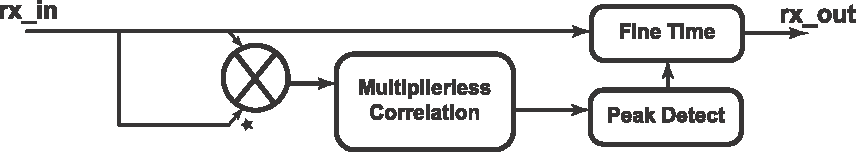
\includegraphics [width=0.9\columnwidth]{Figures/MSCR_RX_STO.pdf}
\caption{The block diagram of fine STO estimation module}
\label{fig:STO}
\end{figure}

\item{Remove Cyclic Prefix:}
\emph{RemoveCP} removes the cyclic prefix attached to each OFDM symbol.
The performance of this module depends on the length of CP $L_{CP}$ specified differently in each standards.
\emph{RemoveCP} consists of a counter to count from the beginning of each symbol and remove the CP samples if the counted value is smaller than $L_{CP}$
This module can be parameterised by adjusting $L_{CP}$ to support multiple standards.

\item{FFT:}
\emph{FFT} is based on the Xilinx FFT/IFFT IP core, but now supports run time reconfiguration of the FFT length according to the underlying selected standard. When the standard is changed, the length of the FFT of this core is reconfigured using the configuration input. The FFT/IFFT IP core reconfiguration is very fast, being able to accomplish a switch within a few clock cycles.

\item{IFO Estimation and Channel Equalisation:}
\emph{IFO\_Est\&Ch\_EstEqu} corrects the IFO and performs channel equalisation. 
IFO results in a cyclic shift in the frequency domain. 
Using differential demodulation of the FFT output, the IFO can be conventionally determined with robustness to frequency selective channels using the correlation function \cite{Park2002} on the second preamble (long preamble) symbol.
The function is expressed as below;

\begin{equation}
\label{integerCFO}
\hat{\epsilon} =\underset{\tilde{\epsilon}}{\operatorname{argmax}}  \left|\sum_{k=0}^{N_{FFT}-1} Y^{*}[k-1] Y[k]  X^{*}[k-\tilde{\epsilon}]  X[k-1-\tilde{\epsilon}]\right|
\end{equation}
where $\epsilon$ denotes the value of IFO, $\hat{\epsilon}$, $\tilde{\epsilon}$ are estimated and trial values of $\epsilon$, respectively,
$Y(k)$ and $X(k)$ denote the $k^{th}$ frequency symbol index of the received subcarriers and the known transmitted preamble, respectively, and the OFDM symbol size $N_{FFT}$ is equal to the FFT size.
The Fig.~\ref{fig:IFO} illustrates the block diagram of IFO estimation and channel equalisation.
The estimated IFO can achieve high precision using cross-correlation in the frequency domain. A low power and low cost IFO estimation architecture presented in Chapter~\ref{chap:CFO} is applied for this module.
\emph{IFO Correction} is performed effectively by cyclic shifting OFDM symbol corresponding to the estimated IFO estimation.

After compensating for IFO, the effects of the channel and residual STO must be taken into account to compensate the received subcarriers.
By employ the information of the second preamble symbol, the effect of the channel can be estimated. 
The estimation and compensation of channel and residual effect can be expressed as below;
\begin{eqnarray}
\label{ChEqu}
Y[k] &=& X[k] * H[k] + N[k] \nonumber \\
H[k] &=& \frac{Y[k]-N[k]}{X[k]} \nonumber \\
\hat{H}[k] &=& \frac{Y[k]}{X[k]}\\
\label{ChCom}
\hat{R}[k] &=& \frac{R[k]}{\hat{H[k]}}
\end{eqnarray}
where $X[k]$, $Y[k]$ are the transmitted and received carriers in the preamble, respectively. 
$H[n]$ represents for the channel and residual STO effect and $N[k]$ is the AWGN.
The equalization taps are estimated in (\ref{ChEqu}), and the compensation for received data carriers is given in (\ref{ChCom}) 
in which $R[k]$, $\hat{R}[k]$ denote received and compensated data carriers, respectively.
Due to symbols are modulated by QPSK, the symbol amplitude is not concerned. So, the complex division of channel estimation and compensation can be equivalently performed by multipling to the conjugation of $X[k]$ and $\hat{H[k]}$, respectively. 
The operation of this module depends on the second preamble that is specified differently in each standard.
Therefore, PR is used for the \emph{IFO\_Est\&Ch\_EstEqu} module to obtain the effective standard-specific implementation.
Suitable precompiled bitstreams are downloaded to the PR module by \emph{CR engine} when the underlying standard is changed.
The PR module must evidently be large enough to contain the largest bitstream among the supported standards.
\begin{figure}
\centering
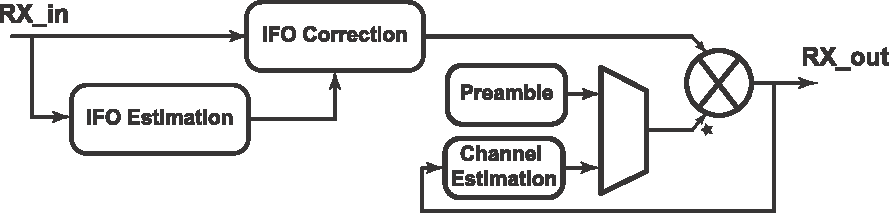
\includegraphics [width=0.9\columnwidth]{Figures/MSCR_RX_IFOCh.pdf}
\caption{The block diagram of IFO estimation and channel equalisation}
\label{fig:IFO}
\end{figure}

\item{Phase Tracking:}
\emph{PhaseTrack} estimates the residual common phase error in each OFDM symbol after channel equalisation. 
The \emph{PhaseTrack} implementation is based on the algorithm presented by Troya et al. \cite{Troya2007}.
The estimation is computed on the pilot symbols inserted in the OFDM symbol. The transmitted pilots are typically assigned
the values \{±1\}. The residual phase error causes a phase rotation on received pilots.
\begin{eqnarray}
\label{PhaseTrack}
P_{k,l} = cos\theta_{l} -\alpha.k.sin \theta_{l} + j (sin\theta_{l} -\alpha.k.cos\theta_{l}),
\end{eqnarray}
where $P_{k,l}$ denotes the phase of received pilot which has frequency index $k$ in the $l^{th}$ OFDM symbol. 
$cos\theta_{l} + j sin\theta_{l}$ is the residual common phase error of the $l^{th}$ OFDM symbol, and $\alpha$ is the slope of the phase distortion.
The residual common phase error is generally estimated for the supported standards as below;
\begin{eqnarray}
\label{CPE}
cos\theta_{l} &=& \frac{1}{N_P} \sum_{k \in S_P} \Re\{P_{k,l}\}, \\ \nonumber
sin\theta_{l} &=& \frac{1}{N_P} \sum_{k \in S_P} \Im\{P_{k,l}\}, \\ \nonumber
\end{eqnarray}
where $N_P$ denotes the number of received pilots employed for estimation, $S_P$ is a set of used pilot frequency indices.
The Fig.~\ref{fig:Phase} shows the block diagram of phase tracking. \emph{Pilot Extract} finds the employed pilots for phase tracking in the OFDM symbol based on allocation vector ($Alloc.~Bits$).
\emph{Phase Accumulator} and \emph{Phase Accumulator} compute the residual common phase error according to (\ref{CPE}).
The phase error is simply compensated for by multiplying the data carriers by the complex conjugate of the estimated common phase error.
To support multiple standards, $N_P$ is parameterised and $S_P$ can be determined through the allocation vector with the value shown in Table~\ref{tab:alloc_vec}

\begin{table}[h]
\centering
\caption{Allocation vector coding.}{
\label{tab:alloc_vec}
\renewcommand{\arraystretch}{1.3}
\begin{tabular}{@{}ll@{}}
\toprule
Subcarrier Type		&  Allocation Bits 	\\ \midrule
Null					&  00				\\
Data				&  10				\\
Positive pilot			&  01				\\
Negative pilot		&  11				\\ 
\end{tabular}
}
\end{table}
\begin{figure}
\centering
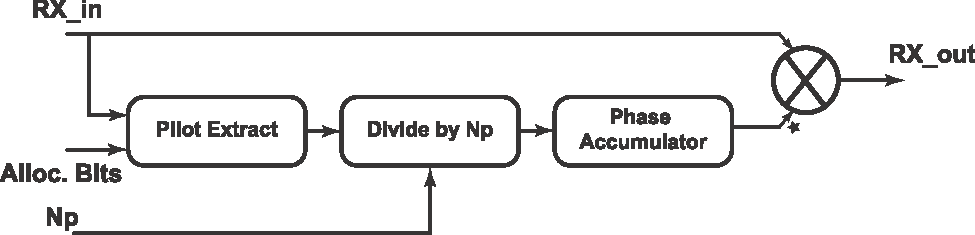
\includegraphics [width=0.9\columnwidth]{Figures/MSCR_RX_Phase.pdf}
\caption{The block diagram of phase tracking module}
\label{fig:Phase}
\end{figure}

\item{Data symbol demodulation (\emph{DatSymDem}):}
At the final step, the received bits are extracted from the data symbol by a data symbol demodulation block named \emph{DatSymDem}. 
In the present implementation, this only supports with QPSK modulation, but can be extended to support different data symbol modulations such as 16-QAM or 64-QAM in future, using the same basic interface.
All data symbols go through this module, and the 2 bits are assigned to the output according to the signed bits of the real and imaginary parts of data symbol.

\end{enumerate}

%---------------------------------------------------------------------------------
\section{Performance Analysis and Discussion}
\label{sec:PerAna}
%---------------------------------------------------------------------------------
\subsection{Analysing the latency and halting time of PR module-based systems}

%\begin{figure*}[!t]
\begin{figure}
\centering{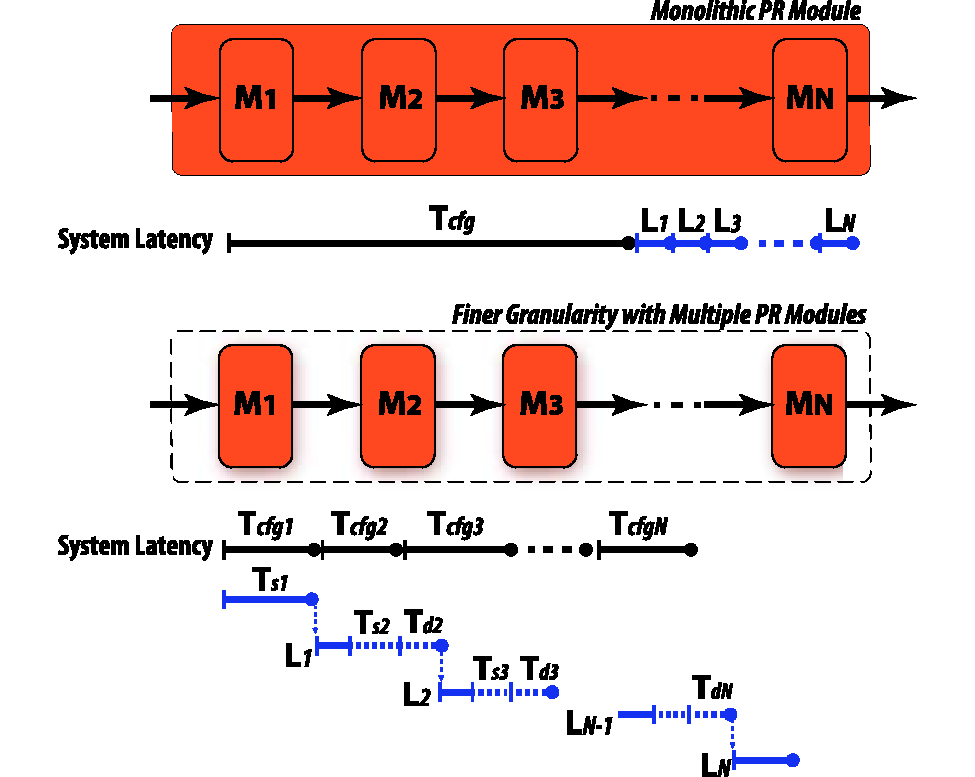
\includegraphics[width=1\columnwidth]{Figures/CRTiming.pdf}}
\caption{Comparison of system latency}
\label{fig:timing}
\end{figure}
 
One crucial challenge when implementing CR systems on reconfigurable hardware is the long adaptation time, including compiling time and reconfiguring time, when changing standards. 
Despite the PR technique can eliminate the compiling time (since PR uses a database of precompiled modules), the partial reconfiguring time is still relatively long, particularly for a large monolithic module. Especially in the case of the CR receiver, the system is halted during reconfiguration, potentially causing the loss of data packet and possibly even the loss of synchronisation. A huge FIFO may be required to store a stream of received samples to overcome the reconfiguration latency when a PR module is reconfigured. A longer reconfiguration time demands a larger FIFO, which results in significantly increased hardware resource and power consumption. Mathematical analysis is used to evaluate the system latency for cases of monolithic PR modules, as well as for a system employing a finer granularity with multiple PR modules, and a mix of PR and parameterized modules for the case when the system switches to a new channel condition. Fig.~\ref{fig:timing} illustrates the system latency for monolithic PR modules and for a system with finer granularity with multiple PR modules. We consider a system consisting of $N$ modules. $T_{c}$ refers to the reconfiguration time. The assumption is that the system or module can not process data during its reconfiguration time. $L_{i}$ is the computation latency of  the $n^{th}$ module. Received data can, of course, be processed during the computation latency. In the case of a large monolithic PR module employed for the system, the system latency, $L_{sys}$, and halting time, $T_{hlt}$ that require a FIFO to buffer the received data which would otherwise be lost, is calculated as follow;

\begin{eqnarray}
\label{Mono}
L_{sys} &=& T_{c} + \sum_{i = 1}^{N}    (L_{i}) \nonumber \\
T_{hlt} &=& T_{c},
\end{eqnarray}
Finer granularity approaches divide the system into multiple sub-modules, each of which employes a PR module. When a module is completely configured, it can process the received data while the following module begins to be configured. Therefore, the system latency and halting time for the case of multiple PR modules can be calculated as follow;

\begin{eqnarray}
\label{Gran}
L_{sys} &=&  \sum_{i = 1}^{N} (T_{ci}) + T_{dN} + L_{N} \nonumber \\
T_{hlt} &=&  \sum_{i = 1}^{N}  (T_{si}),
\end{eqnarray}
where $T_{di}$ refers the processing delay of the following module and $T_{si}$ is the stalling time to wait for configuration of the following module. If the computation latency of a module, $L_{i}$, is greater than the reconfiguration time of the following module,  $T_{ci+1}$, the following module has to delay operation by a duration $T_{di}$ before it receives input data for processing. Otherwise, the previous modules is halted a duration $T_{si}$ until the following module is completely configured. The following module begins processing data just after its configuration is done ($T_{di} = 0$). 

\begin{equation}
\label{DelayTime}
T_{di} = \begin{cases} Max(T_{ci}, T_{di-1}+L_{i-1}) - T_{ci}  	& i = 2..N, \\ 
						0 										& i = 1 \end{cases}  \\ 
\end{equation}
\begin{equation}
\label{HaltTime}
T_{si} = \begin{cases} T_{ci} - min(T_{ci}, T_{di-1}+L_{i-1}), 	&  i = 2..N, \\ 
					  T_{c1}									&  i=1 \end{cases}  \\ 
\end{equation}

Substituting the above equations into (\ref{Gran}), 
\begin{eqnarray}
\label{Gran2}
L_{sys} &= & \sum_{i = 1}^{N}(T_{ci}) + L_{N} +   \nonumber \\
		& & (Max(T_{cN}, (Max( ... ) - T_{cN-1}) + L_{N-1}) - T_{cN})  \nonumber \\
T_{hlt} &= &\sum_{i = 1}^{N}(T_{ci})  -  \sum_{i = 2}^{N}  (min(T_{ci}, T_{di-1}+L_{i-1})),
\end{eqnarray}

As can be seen in the equations, the system latency and halting time in the case of multiple PR modules are theoretically reduced thanks to being able to overlap the reconfiguration and data processing periods. Practically, the reconfiguration times usually are much greater than the processing latencies. This leads to $T_{di} = 0$ and  $min(T_{ci}, T_{di-1}+L_{i-1}) = L_{i-1}$ resulting in the approximated equations for (\ref{Gran2}) as below;  
\begin{eqnarray}
\label{Gran3}
L_{sys} &= & \sum_{i = 1}^{N}(T_{ci}) + L_{N}    \nonumber \\
T_{hlt} &=  &\sum_{i = 1}^{N}(T_{ci})  -  \sum_{i = 1}^{N-1}  (L_{i}),
\end{eqnarray}

In addition, because of the optimisation in hardware compilation, the overhead of partitioning into multiple PR modules leads to the fact that $\sum_{i = 1}^{N}(T_{ci})$ is clearly greater than $T_{c}$, in (\ref{Mono}). Therefore, the system latency, $L_{sys}$, and halting time, $T_{hlt}$ in (\ref{Gran2}) may be greater than that in (\ref{Mono}).
Generally, the finer granularity approach can only achieve the efficiency in terms of the system latency and halting time, if the gain of overlapping the reconfiguration and data processing is greater than the overhead of partitioning into multiple PR modules.

Through the above analyses and comparison of large monolithic PR modules with a finer granularity approach, we proposed a new method employing a mix of PR modules and parameterised modules to obtain a significant reduction in system latency and halting time. Each module in the processing chain of the granularity approach is investigated, and commonalities across different operation modes are analysed. For modules requiring only minor modifications, parameterized versions are created.
For the $i^{th}$ module to be parameterised, the configuration time of this module can be eliminated because the parameterised modules can switch operation mode within one clock period. This approximately results in the following simplified equations;
\begin{eqnarray}
\label{Pro}
T_{ci} &\approx & 0   \nonumber \\
T_{si} &\approx & 0 \nonumber \\
T_{di} &\approx & T_{di-1} +  L_{i-1},
\end{eqnarray}

The above equations show the increasing efficiency of overlapping the performing reconfiguration and data processing leading to significant reduction in the system latency and halting time.

\subsection{Analysing results of proposed OFDM-based MSCR architecture}
The system latency and halting time of OFDM-based MSCR systems are investigated based on the results of hardware consumption and system performance when implemented on a Vertex6 FPGA (XC6VLX240t). 
A comparison of large monolithic PR module, finer granularity and proposed approaches is given to show the advantages of the proposed architecture. 
To compute a configuration time of a PR module, the bitstreams of all implementations have to be computed. 
The area of the PR module, i.e., the occupied and reserved hardware resources, must satisfy the needs of the largest implementation. 
For the monolithic PR module approach, it is required that the PR module must be able to contain the 802.22 OFDM-based  implementation, which is the largest receiver implementation among the three target implementations. Similarly to granularity approach, the configurations of the PR modules are computed based on the sub-modules of the 802.22 OFDM-based  implementation.
Table~\ref{tab:Resouces} reports the hardware resources usage of each sub-module and transmitter, receiver system for 802.22 on the Vertex6 FPGA (XC6VLX240t). $M_1$, $M_2$, $M_3$, $M_4$, $M_5$, $M_6$, $M_7$, $M_8$  denote the functional modules of the OFDM based system: synchronisation, frequency compensation, fine STO estimation, remove CP, FFT, IFO estimation and channel equalisation, phase tracking, data symbol demodulation, respectively. $M_R$, $M_T$ are the monolithic receiver and transmitter sub-systems, respectively.
%Because we employ the multiplyless correlation for Fine STO estimation, DSP blocks are not used in this module but resulting in increased number of used slides. 
These results are employed to calculate the bitstream size of PR modules for each functional block. Fig.~\ref{fig:Bitstream} illustrates the bitstream sizes of each PR module, that are employed to calculate the configuration time later. The bitstream sizes of PR module for the functional modules are relatively small compared to the monolithic PR module for the receiver sub-system. The $M_3$ bitstream is the largest bitstream among the functional granular modules. Interestingly, the bitstream of the receiver sub-system is nearly triple that of the transmitter sub-system.
\begin{table}[hb]
	\centering
	\caption{Resources for 802.22 OFDM-based implementation}
	\label{tab:Resouces}
	\begin{tabular}{l|c|c|c}
        \hline \hline
    			  \makebox[1.2cm][c]{$modules$}	&  \makebox[1cm][c]{Slices}  &  {DSP} &  {BRAM} \\
	\hline
		$M_1$(\textit{Synch})     				& 498 		& 5	& 0 \\
		$M_2$(\textit{FreComp})				& 474		& 4 	& 0 \\
		$M_3$(\textit{FineSTO\_Est})			& 2414	& 0 	& 0 \\
		$M_4$(\textit{RemoveCP})			& 23  		& 0	& 0 \\
		$M_5$(\textit{FFT})	  			& 1179  	& 15	& 11 \\
		$M_6$(\textit{IFO\_Est\&Ch\_EstEqu})	  	& 1249 	& 6	& 0 \\
		$M_7$(\textit{Phasetrack})	  		& 523  	& 3	& 0 \\
		$M_8$(\textit{DatSymDem})	  		& 4	  	& 0	& 0 \\
		$M_R$(Receiver)  					& 6363  	& 33	& 11 \\
		$M_T$(Transmitter)					& 1668  	& 15	& 11 \\
	\hline \hline
    \end{tabular}
\end{table}

\begin{figure}
\centering
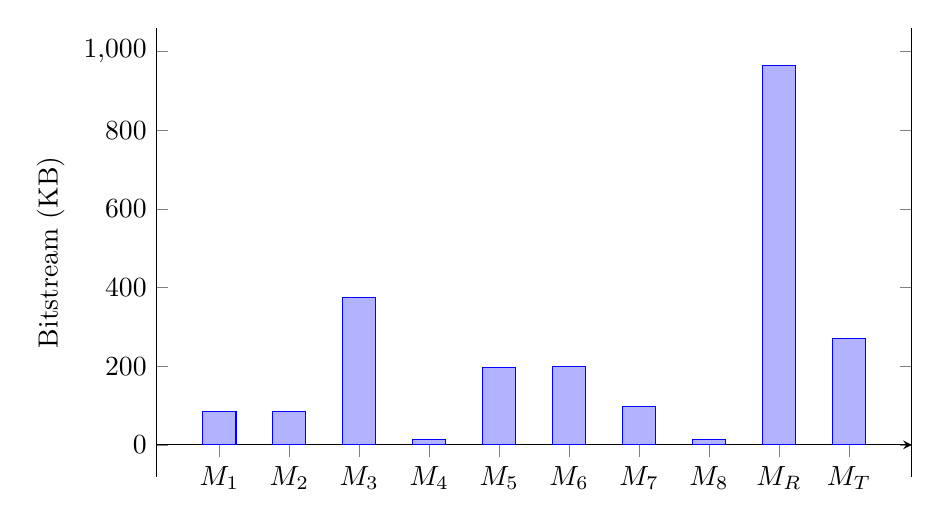
\begin{tikzpicture}[scale=1]
        \begin{axis}[
           axis x line=center,
           bar width=12pt,
           symbolic x coords={ $M_1$,$M_2$,$M_3$,$M_4$,$M_5$,$M_6$, $M_7$, $M_8$, $M_R$, $M_T$ },
           xtick=data,	
	enlargelimits=true,
	ylabel={Bitstream (KB)},
	ylabel style={align=center},  
%	xlabel={PR modules},
	ybar, x post scale=1.4]
            \addplot coordinates {
                ($M_1$,84.03) ($M_2$,84.03) ($M_3$,374.91) ($M_4$,14.54) ($M_5$,197.15) ($M_6$, 200.38)
                ($M_7$, 98.58) ($M_8$, 14.54) ($M_R$, 964.75) ($M_T$, 269.87)                
               };
        \end{axis}
    \end{tikzpicture}
\caption{The bitstream size of PR modules}
\label{fig:Bitstream}
\end{figure}

The latencies of functional modules are considered for three standards. Fig.~\ref{fig:Latency} shows the latencies in number of clock cycles. As can be seen, the latencies for the 802.11 standard are smallest, because this standard uses the shortest FFT length, i.e., shortest symbol length for OFDM modulation. It should be noted that during the latency time the module still receives input data for processing. The processing chain is halted when the latency time has ended but the reconfiguration of the following module has not been completed yet. Therefore, the worst case halting time is a case of the shortest latency and the longest reconfiguration time. So, the latencies for 802.11 are taken to calculate the system halting time. The latency of the synchronisation module depends on the timing offset that is the duration from the time of receiving input samples to the time when the first sample of the coming frame is received. The synchronisation module does not output data if no frame is detected. Generally, the synchronisation latency is calculated as $L_{1} = Offset + processing time$.  To solely evaluate the processing latency of the synchronisation module, the timing offset is considered to equal 0. We will consider the presence of timing offset later for calculating the system halting time and FIFO requirement.
\begin{figure}
\centering
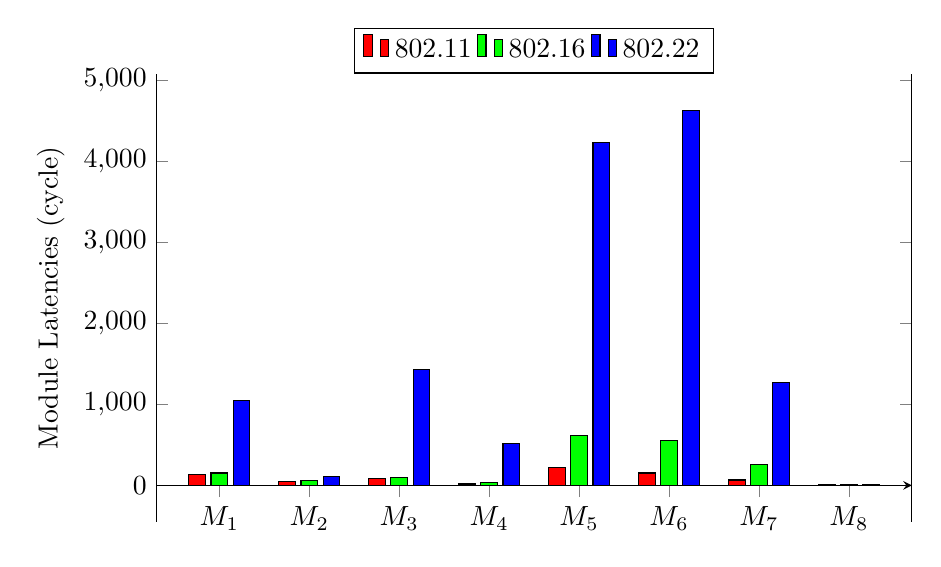
\begin{tikzpicture}
        \begin{axis}[
           ylabel={Module Latencies (cycle)},         
	ylabel style={align=center},           
           xtick = data,	
	axis x line=center,
           bar width= 6pt,
%	nodes near coords,
	legend style={at={(0.5, 1)}, anchor=south, legend columns=-1},
           symbolic x coords={$M_1$,$M_2$,$M_3$,$M_4$,$M_5$,$M_6$, $M_7$, $M_8$ },
	enlargelimits=true,
  	ybar, x post scale=1.4]
	\addplot[fill=red] coordinates {
		($M_1$,137) ($M_2$,45) ($M_3$,84) ($M_4$,17) ($M_5$,216) ($M_6$, 153) ($M_7$, 66) ($M_8$,11) 
           };
	\addplot[fill=green] coordinates {
		($M_1$,153) ($M_2$,61) ($M_3$,100) ($M_4$,33) ($M_5$,616) ($M_6$, 553) ($M_7$, 252) ($M_8$,11) 
           };
 	\addplot[fill=blue] coordinates {
		($M_1$,1048) ($M_2$,110) ($M_3$,1428) ($M_4$,513) ($M_5$,4226) ($M_6$, 4617) ($M_7$, 1273) ($M_8$,11) 
            };
   	\legend{802.11, 802.16, 802.22}
        \end{axis}
\end{tikzpicture}
\caption{The latency of sub-modules for three standards}
\label{fig:Latency}
\end{figure}

The partial reconfiguration is performed with the ICAP interface that supports downloading speeds of up to 400~MBps. 
Practically, because of the overhead of PR controller, a speed of 380~MBps is used for downloading the PR bitstream to FPGA.
Therefore, the accuracy of computing the reconfiguration time for PR modules by dividing the bitstream size by the downloading speed should be acceptable.
In addition, the sampling frequency for the radio signal is varied according to the currently chosen standard. 
We use a sampling frequency of 10 MHz (i.e., the clock period = 0.1 us) that is typically defined for the 802.11p standard.
The latency is calculated from the results of 802.11 standard in Fig.~\ref{fig:Latency} multiplied by the clock period of 0.1 us.
Fig.~\ref{fig:CfgLat} illustrates the time of configuration and latency for each module. 
The values of latency are scaled by a factor of 10 for better observation. As can be seen, the latency is very small in comparison to the configuration time. 
It is clearly not efficient to perform the overlapping reconfiguration and data processing. Therefore, the finer granularity approach may not obtain a good improvement.
\begin{figure}
\centering
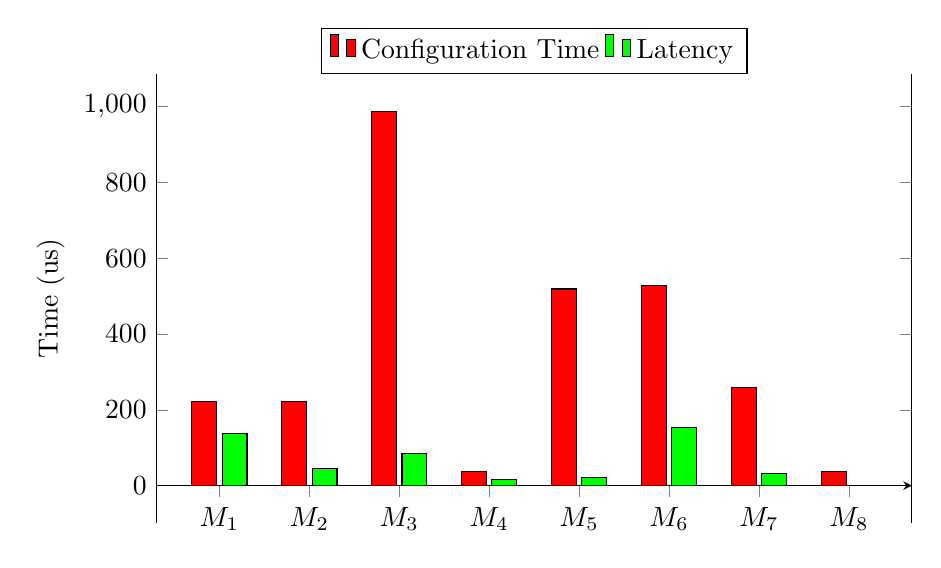
\begin{tikzpicture}
        \begin{axis}[
           ylabel={Time (us)},         
	ylabel style={align=center},           
           xtick = data,	
	axis x line=center,
           bar width= 9pt,
%	nodes near coords,
	legend style={at={(0.5, 1)}, anchor=south, legend columns=-1},
           symbolic x coords={$M_1$,$M_2$,$M_3$,$M_4$,$M_5$,$M_6$, $M_7$, $M_8$ },
	enlargelimits=true,
  	ybar, x post scale=1.4]
	\addplot[fill=red] coordinates {
		($M_1$,221.14) ($M_2$,221.14) ($M_3$, 986.61) ($M_4$, 38.27) ($M_5$, 518.82) ($M_6$, 527.33) ($M_7$, 259.41) ($M_8$,38.27)  
           };
	\addplot[fill=green] coordinates {
		($M_1$,137) ($M_2$,45) ($M_3$, 84) ($M_4$, 17) ($M_5$, 21.6) ($M_6$, 153) ($M_7$, 33) ($M_8$, 01)  
           };
	\legend{Configuration Time, Latency}
        \end{axis}
\end{tikzpicture}
\caption{The configuration time and latency of sub-modules for OFDM-based MSCR system}
\label{fig:CfgLat}
\end{figure}

The system halting time is an accumulated value of the halting time in each module described in (\ref{HaltTime}). During the halting time, the processing chain is halted and a FIFO is required to buffer input samples. Because the halting time of the synchronisation module depends on the time when a new frame is detected. The timing offset must be taken into account. Given a scenario of a transmission, shown in Fig.~\ref{fig:tx-rx} when a standard switch is required, Both the transmitter and receiver spend time to reconfigure the system for the new operating standard. In the proposed receiver, the synchronisation module is a parameterised module, so this module can change its function very fast - within one clock period and hence quickly process input samples. However, a new frame is not able to be sent so quickly because the transmitter is still being reconfigured, resulting in a timing offset in the receiver. It is thus reasonable that the minimum timing offset can be chosen as the configuration time of the transmitter whose hardware characteristics were reported in Table~\ref{tab:Resouces}.
\begin{figure}
\centering
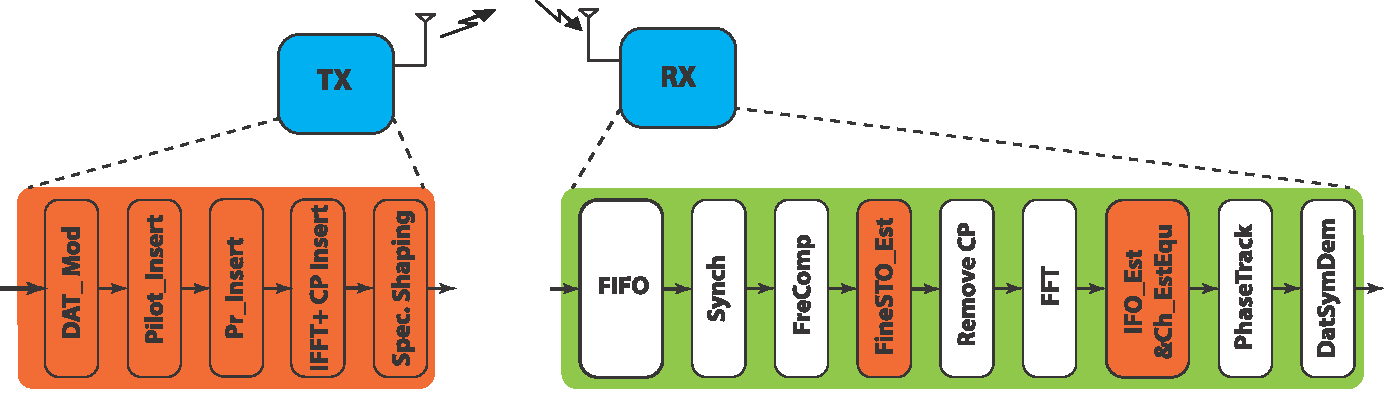
\includegraphics [width=1\columnwidth]{Figures/CR_Tx-Rx.pdf}
\caption{A scenario of a transmission}
\label{fig:tx-rx}
\end{figure}

\definecolor{M1}{HTML}{17191C}
\definecolor{M2}{HTML}{67899C}
\definecolor{M3}{HTML}{37793C}
\definecolor{M4}{HTML}{77698C}
\definecolor{M5}{HTML}{57595C}
\definecolor{M6}{HTML}{27497C}
\definecolor{M7}{HTML}{77392C}
\definecolor{M8}{HTML}{47296C}
\definecolor{MR}{HTML}{91194C}
\begin{figure}
\centering
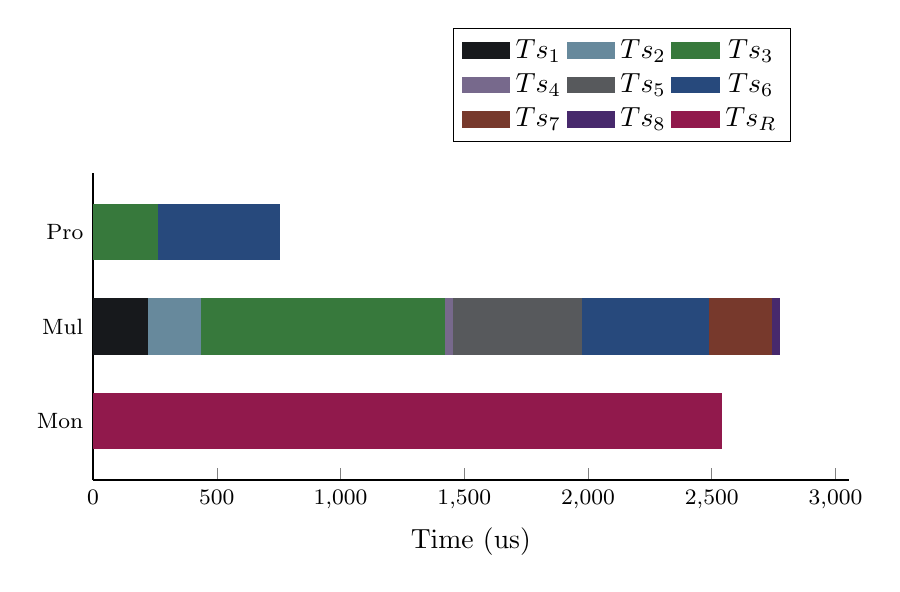
\begin{tikzpicture}
\begin{axis}[
	xbar stacked,
	legend style={at={(0.7, 1.1)}, anchor=south, legend columns=3},
    	ytick=data,
    	axis y line*=none,
    	axis x line*=bottom,
	tick label style={font=\footnotesize},
    	bar width= 20pt,
    	xlabel={Time (us)},
    	yticklabels={Mon, Mul , Pro},
    	xmin=0,
%    	xmax=600,
    	area legend,
    	y=12mm,
    	enlarge y limits={abs=0.625}, x post scale=1.4
	]
	\addplot [M1,fill=M1] coordinates {(0,0) (221.14,1) (0 ,2) };
	\addplot [M2,fill=M2] coordinates {(0,0) (214.28,1) (0,2) };
	\addplot [M3,fill=M3] coordinates {(0,0) (984.36,1) (258.22,2) };
	\addplot [M4,fill=M4] coordinates {(0,0) (034.07,1) (0,2) };
	\addplot [M5,fill=M5] coordinates {(0,0) (517.97,1) (0,2) };
	\addplot [M6,fill=M6] coordinates {(0,0) (516.53,1) (495.63,2) };
	\addplot [M7,fill=M7] coordinates {(0,0) (251.76,1) (0,2) };
	\addplot [M8,fill=M8] coordinates {(0,0) (034.97,1) (0,2) };
	\addplot [MR,fill=MR] coordinates {(2538.82,0) (0,1) (0,2)};
	\legend{$Ts_1$,$Ts_2$,$Ts_3$,$Ts_4$,$Ts_5$,$Ts_6$, $Ts_7$, $Ts_8$ , $Ts_R$}
\end{axis}  
\end{tikzpicture}
\caption{ The halting time comparison of the system for three different approaches }
\label{fig:Halt}
\end{figure}

Fig.~\ref{fig:Halt} shows the system halting time of the three approaches. $Mon$, $Mul$, $Pro$ denote the halting time of the monolithic PR module approach, the multiple PR module approach, and the proposed approach, respectively.
$Ts_n$ is the halting time of the corresponding $M_n$ functional module. $Ts_R$ is the halting time of the monolithic receiver sub-system. As can be seen, the halting time of the multiple PR module approach is greater compared to the monolithic PR module approach, because the gain achieved by overlapping the reconfiguration and data processing is greater compared to the overhead of partitioning into multiple PR modules. The proposed approach can significantly reduce the halting time that only less than one-third of that of the monolithic PR module approach. This results in a reduction in the FIFO requirement.

\begin{figure}	
\centering
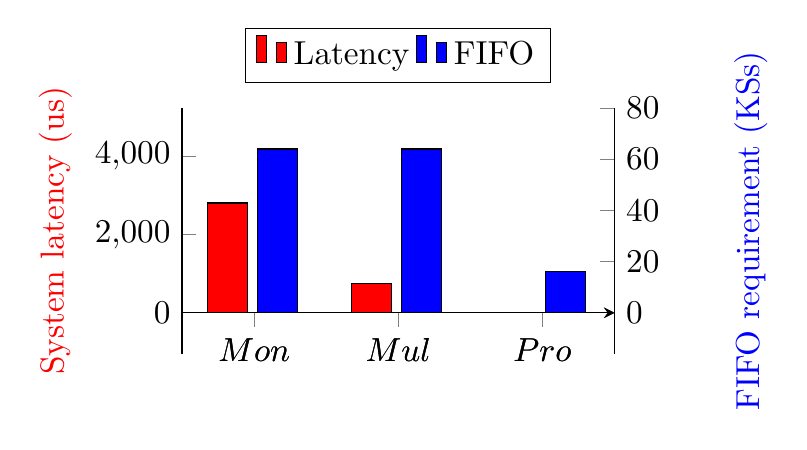
\begin{tikzpicture}[scale=1.2]
 	\begin{axis}[
           ylabel={System latency (us)},         
	ylabel style={align=center, color=red},           
 	ymin=0,
	width= 0.4*\textwidth,
           xtick = data,	
	axis x line=center,
           bar width= 12pt,
           symbolic x coords={0, $Mon$, $Mul$, $Pro$, $$},
	enlargelimits=0.25,
    	axis y line*=none,
  	ybar, x post scale=1.4]
	\addplot[fill=red,shift={(-8pt,0)}] coordinates {($Mon$,4190.82) ($Mul$,2811.12) ($Pro$,753.97)  };
 	\end{axis}
 
	\begin{axis}[
           ylabel={FIFO requirement (KSs)},         
	ylabel style={at={(1.25,0.5)}, color=blue},       
 	ymin=0,
	width= 0.4*\textwidth,
           xtick = data,	
	axis x line=center,
           bar width= 12pt,
	legend style={at={(0.5, 1.1)}, anchor=south, legend columns=2},
           symbolic x coords={0, $Mon$, $Mul$, $Pro$, 1},
	enlargelimits=0.25,
	axis y line*=right,
  	ybar, x post scale=1.4]
	\addplot [fill=red] coordinates {($Mon$,0) ($Mul$,0) ($Pro$,0) }; 
	\addplot [fill=blue] coordinates {($Mon$,64) ($Mul$,64) ($Pro$,16)  };
 	\legend{Latency, FIFO}
 	\end{axis}
      
\end{tikzpicture}
\caption{A comparison of the three approaches in terms of system latency and FIFO requirement}
\label{fig:LatFIFO}
\end{figure}

Fig.~\ref{fig:Halt} compares the three approaches in terms of system latency and the FIFO requirement to avoid losing data frame. The system latencies are computed in the worst case which is the latencies for the 802.22 standard (the longest latencies). The FIFO requirement is calculated based on multiplying the sampling frequency by the halting time, followed by rounding up to the next power of two value. The system latency of the proposed method is significantly reduced to 18~\% and 27~\% of the system latency of the monolithic PR module approach and the multiple PR module approach, respectively. The FIFO requirement for the proposed approach is only 16 kilo-samples (KSs) while the two other approaches require a FIFO which must store up to 64~KSs.

%---------------------------------------------------------------------------------
\section{Summary}
%---------------------------------------------------------------------------------
Our research explores the feasibility of designing efficient multi-standard radios to enhance bandwidth efficiency and avoid spectrum congestion. 
Our proposed architecture assumes the use of OFDM radio, and implemented on an FPGA, coupling parameterized modules and PR modules to achieve flexibility while minimizing reconfiguration time.
A mathematical analyses of the FPGA synthesis results shows that the proposed architecture achieves a significant reduction of 82~\% compared to conventional approaches in terms of system latency. 
The FIFO requirement of the proposed method is also decreased to 25~\% of that required for the conventional method.
The work presented in this chapter has been submitted in [J5].